\documentclass[10pt,oneside,slovak,a4paper]{article}

\usepackage[slovak]{babel}

\usepackage[IL2]{fontenc} 
\usepackage[utf8]{inputenc}
\usepackage{graphicx}
\usepackage{listings}
\usepackage{verbatim}
\usepackage{url}
\usepackage{amsfonts}
\usepackage{hyperref} 
\usepackage{cite}
\usepackage[margin=1.3in]{geometry}

\setlength{\tabcolsep}{18pt}
\renewcommand{\arraystretch}{1.5}

\lstset{literate=%
         {á}{{\'a}}1
         {í}{{\'i}}1
         {é}{{\'e}}1
         {ý}{{\'y}}1
         {ú}{{\'u}}1
         {ó}{{\'o}}1
         {ě}{{\v{e}}}1
         {š}{{\v{s}}}1
         {č}{{\v{c}}}1
         {ľ}{{\v{l}}}1
         {ř}{{\v{r}}}1
         {ž}{{\v{z}}}1
         {ď}{{\v{d}}}1
         {ť}{{\v{t}}}1
         {ň}{{\v{n}}}1                
         {ů}{{\r{u}}}1
         {Á}{{\'A}}1
         {Í}{{\'I}}1
         {É}{{\'E}}1
         {Ý}{{\'Y}}1
         {Ú}{{\'U}}1
         {Ó}{{\'O}}1
         {Ě}{{\v{E}}}1
         {Š}{{\v{S}}}1
         {Č}{{\v{C}}}1
         {Ř}{{\v{R}}}1
         {Ž}{{\v{Z}}}1
         {Ď}{{\v{D}}}1
         {Ť}{{\v{T}}}1
         {Ň}{{\v{N}}}1                
         {Ů}{{\r{U}}}1
         {Ä}{{\"A}}1
         {Ľ}{{\v{L}}}1
         {ä}{{\"a}}1    
}

\pagestyle{headings}


\begin{document}

\begin{titlepage}
	\centering
	\par\vspace{1cm}
	{\scshape\LARGE Slovenská technická univerzita v Bratislave \par}
	{\scshape\Large Fakulta informatiky a informačných technológií\par}
	\vspace{1.5cm}
	{\large Princípy informačných systémov \par}
	{\large Dokumentácia projektu\par}
	\vspace{5cm}
	{\huge\bfseries Repozitár - digitálna knižnica\par}
	\vspace{0.5cm}
	{\Large\itshape Martin Staňo, Veronika Včelková, Dávid Kubík\par}
	\vfill
	cvičiaci\par
	RNDr. Marta \textsc{Gnipová}, Ing. Nadežda \textsc{Andrejčíková}, PhD.\par
	\vspace{1cm}
	{\large \today\par}
\end{titlepage}

\tableofcontents

\newpage


\section{Percentuálny podiel práce autov na projekte}

\vspace{1cm}

\begin{tabular}{ |p{3cm}||p{2.5cm}|p{3cm}|p{2.5cm}|}
 \hline
 \multicolumn{4}{|c|}{\textbf{Podiel práce}} \\
 \hline
 Časť projektu & Martin Staňo & Veronika Včelková & Dávid Kubík\\
 \hline
 Počiatočný návrh a identifikácia úloh & 0 & 0 &  0\\
 \hline
 Zapracovanie pripomienok z konzultácií a vytvorenie návrhu v IBM BPM & 0 & 0 &  0\\
 \hline
 Návrh formulárov & 0 & 0 &  0\\
 \hline
 Návrh použitia webových služieb & 0 & 0 &  0\\
 \hline
 Implementácia v IBM BPM & 0 & 0 &  0\\
 \hline
 Vypracovanie dokumentácie & 0 & 0 &  0\\
 
 \hline
\end{tabular}

\newpage

\section{Špecifikácia projektu: Repozitár - digitálna knižnica}

\subsection{Úvod}

Cieľom tohto projektu je definovať biznis procesy na podporu nižšie popísanej problémovej domény. Tieto biznis procesy budu navrhnuté, implementované a otestované v prostredí IBM BPM. Pri návrhu a implementácií biznis procesov sa dbalo na dodržiavanie princípov SOA (využívanie webových služieb a ich správne prepojenie).


\subsection{Zadanie - špecifikácia}

Horizont H2020 určuje vedeckovýskumným pracoviskám povinnosť evidovať svoje publikované výsledky VaV v repozitári – vlastnom, konzorcionálnom, národnom. Údaje, ktoré popisujú dokument – bibliografický záznam, môže vykonávať spracovateľ, knihovník, alebo priamo vedec.

Formulár obsahuje minimálne všetky základné údaje nevyhnutné pre jednoznačnú identifikáciu daného typu dokumentu. Pri vkladaní dát sú priebežne systémom vykonávané viaceré kontroly, dôležité je, aby všetky entity boli identifikovaný perzistentným jedno-jednoznačným identifikátorom, teda aby v systéme nemohli na základe termínu reprezentujúceho dané idivídum vznikať homonymá, ale zároveň aby systém vedel k danému termínu agregovať všetky jeho synonymá, akronymy, či iné variantné formy termínov, ktoré môžu vystihovať význam tohto indivídua.

Zadané údaje sa vždy uložia do systému aj s prípadnými chybami, všetky údaje sú logované a v prípade, že neexistuje identifikátor pre dané indivídum entity, systém vytvorí nový záznam pre toto individum a pridelí mu požadovaný identifikátor a následne vo formulári prelinkuje na tento identifikátor.

Všetky vzťahy medzi entitami sú evidované na základe významu a prostredníctvom uvedených identifikátorov, teda nie odkaz na termín, ten sa generuje následne prostredníctvom daného identifikátora z príslušnej databázy modelu. 

Konečnú platnosť a správnosť údajov, môže potvrdiť až knihovník, vtedy sa všetky údaje pre iný používateľov a teda aj autorov stávajú len read/only, návrh na akúkoľvek zmenu môžu vykonať len prostredníctvom mailu, alebo poznámky k záznamu. Ak údaje vkladá spracovateľ, alebo vedecký pracovník, ostatní spoluautori ako aj konkrétny spracovateľ sú o tom informovaní , rovnako ako aj v prípade, keď knihovník potvrdí správnosť a zverejní záznam. 

Samozrejme autori určujú podmienky, pre koho bude záznam aj dokument dostupný voľne a pre ktoré skupiny na vyžiadanie, prípadne pre koho zasa úplne neviditeľný, pričom môže toto kombinovať aj s časovým určením, teda napr. pre pracovníkov oddelenia voľne dostupný pre ostatných akademických a vedecko-pedagogických pracovníkov voľne dostupný po 2 rokoch a pre ostatných viditeľný po 3 a voľne dostupný po 5 rokoch.

Navrhnite procesy, ktoré umožnia spracovať a sprístupňovať repozitár publikovaných výsledkov vedy a výskumu tak, že bude zároveň evidovať všetky vzájomné vzťahy medzi entitami použitými pre popis publikovaného výsledku VaV na základe významu.

\newpage

\section{Návrh, analýza a opis biznis procesov}

V tomto projekte budú analyzované a implementované nasledujúce biznis procesy súvisiace s problémovou doménou:

\begin{itemize}
\item Nahranie bibliografického záznamu
\item Aktualizácia bibliografického záznamu
\item Vyhľadanie bibliografického záznamu
\end{itemize}

\subsection{Dátový model}

Vo vyššie pomenovaných biznis procesoch sme identifikovali nasledujúce entity ako aj ich atribúty a vzťahy medzi nimi. Tieto entity zároveň reprezentujú naše biznis objekty (komplexné dátové typy).

\begin{figure}[h]
\label{datamodel}
\centering
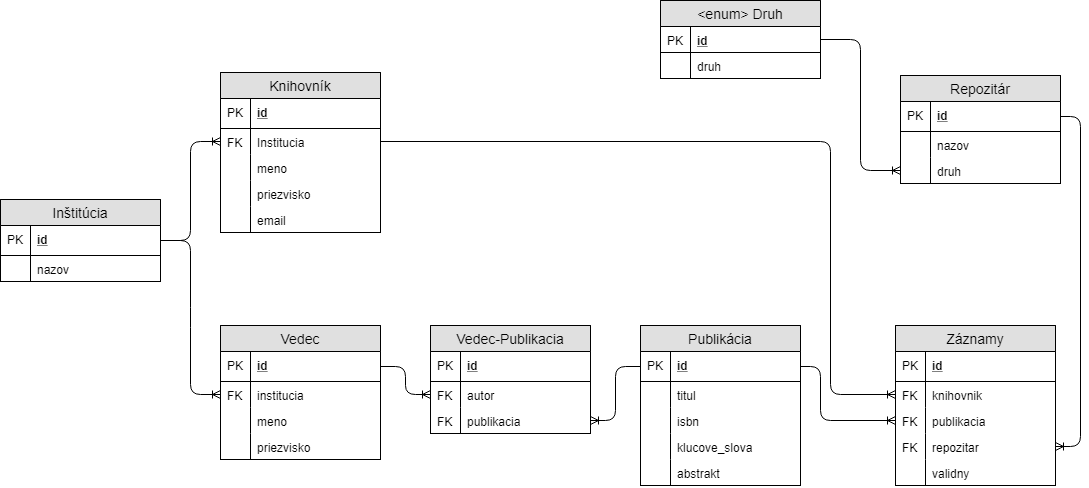
\includegraphics[scale=0.4]{datovymodel.png} 
\caption{ER diagram dátového modelu}
\end{figure}

\subsection{Nahranie bibliografického záznamu}

\subsection{Opis}

Cieľom tohto biznis procesu je nahranie bibliografického záznamu do konkrétneho repozitára. Vedecký pracovník vyplní detaily bibliografického záznamu. Knihovník






\end{document}